\documentclass[tikz,border=2pt]{standalone}
\usepackage{amsmath,amssymb}
\usepackage{tikz}

\begin{document}
% An exterior point has a whole ball outside E (disjoint from E). Interior, boundary and
% exterior split the space into three parts.
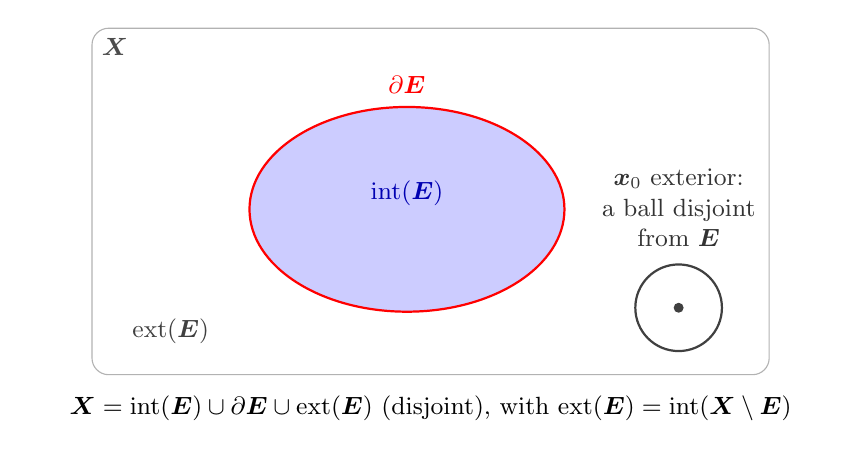
\begin{tikzpicture}[every node/.style={font=\small}]
	\draw[gray!60, rounded corners=6pt] (-4,-2.1) rectangle (4.6,2.3);
	\node[gray!60!black, anchor=north west] at (-4,2.3) {$\boldsymbol{X}$};
	\fill[blue!20] (0,0) ellipse (2.0 and 1.3);
	\draw[red, thick] (0,0) ellipse (2.0 and 1.3);
	\node[blue!70!black] at (0,0.2) {$\operatorname{int}(\boldsymbol{E})$};
	\node[red, anchor=south] at (0,1.35) {$\partial\boldsymbol{E}$};
	\node[gray!50!black] at (-3.0,-1.55) {$\operatorname{ext}(\boldsymbol{E})$};
	\fill[gray!50!black] (3.45,-1.25) circle (1.8pt);
	\draw[gray!50!black, thick] (3.45,-1.25) circle (0.55);
	\node[gray!40!black, anchor=south, align=center] at (3.45,-0.6) {$\boldsymbol{x}_0$ exterior:\\ a ball disjoint\\ from $\boldsymbol{E}$};
	\node[anchor=north, align=flush center, text width=10cm] at (0.3,-2.25) {$\boldsymbol{X}=\operatorname{int}(\boldsymbol{E})\cup\partial\boldsymbol{E}\cup\operatorname{ext}(\boldsymbol{E})$ (disjoint), with $\operatorname{ext}(\boldsymbol{E})=\operatorname{int}(\boldsymbol{X}\setminus\boldsymbol{E})$};
\end{tikzpicture}
\end{document}
